\documentclass{article}
\usepackage[letterpaper, margin=1in]{geometry}
\usepackage{fixltx2e}
\usepackage{listings}
\usepackage{graphicx} % Required for inserting images
\usepackage{setspace}
\usepackage{multirow}
\usepackage{float}
\usepackage[sorting=none]{biblatex}
\addbibresource{labreport.bib}

\setstretch{1.50}
\title{
\textbf{Laboratory Report} \\
\large Core-affine threaded interpolating elevation of a \emph{n $\times$ n} matrix \emph{M} given a lower resolution digital elevation matrix \emph{N}
}
\author{Jasrel Roby Peralta}
\date{May 2023}

\sloppy
\begin{document}

\maketitle

\section*{Introduction}
\hspace{\parindent} After creating a threaded computer program from Exercise 02, use the programming exercise from Exercise 03 to record average runtimes of estimation of a \emph{n $\times$ n} matrix when using a different \emph{t} number of threads.

\section*{Objectives}
The goal for this exercise is the following:
\begin{itemize}
    \item determine the complexity of estimating the point elevation of a \emph{n $\times$ n} square matrix with randomized values at grid points divisible by 10 when using \emph{n} concurrent processors and other values of concurrent processors.
    \item see if the runtime for this exercise is lower than the average runtime that was obtained in Exercise 01 and Exercise 02.
    \item figure out why higher values of \emph{n} size of matrix are now faster using \emph{t} concurrent cores.
\end{itemize}

\section*{Methodology}
\hspace{\parindent} The machine used for this exercise is running on Ubuntu 22.04.2 LTS x86\_64, Intel i-7 8700 (12 cores) @ 4.60GHz, AMD ATI Radeon HD 8570 / RS 430, with 16GB memory. The programming language used in the computer program is Python 3.10.6. The interpolating algorithm used was the Federal Communications Commission (FCC) method. The graphing software used for making the charts is LibreOffice Calc. \\
\indent The computer program made use of the \emph{multiprocessing} module of Python 3.10.6, to utilize \emph{t} cores and concurrently estimate different \emph{(n/t) $\times$ n} submatrices from the \emph{n $\times$ n} matrix. \\ 
\indent The size of the matrix for all recorded runs was n = 8000. Moreover, three (3) runs were done using \emph{t} number of threads, starting from 1 (2\textsuperscript{0}) up to 64 (2\textsuperscript{6}). The created threads are then automatically assigned by Python to different cores. These runs were then averaged and recorded to a table.
\indent The program was further analyzed using \emph{htop}, an interactive process viewer, to see if the cores being assigned are being used to its full capacity.

\section*{Results and Discussion}
\hspace{\parindent} After running the code three (3) successive times, using \emph{n} matrix size and \emph{t} cores, the following table is produced:

\begin{table}[H]
    \centering
    \noindent\makebox[\textwidth]{
    \begin{tabular}{|c|c|ccc|c|}
    \hline
    \multirow{2}{*}{\textbf{\begin{tabular}[c]{@{}c@{}}n\\ (size of matrix)\end{tabular}}} & \multirow{2}{*}{\textbf{\begin{tabular}[c]{@{}c@{}}t\\ (number of concurrent cores)\end{tabular}}} & \multicolumn{3}{c|}{\textbf{\begin{tabular}[c]{@{}c@{}}Time Elapsed\\ (seconds)\end{tabular}}} & \multirow{2}{*}{\textbf{\begin{tabular}[c]{@{}c@{}}Average Runtime\\ (seconds\end{tabular}}} \\ \cline{3-5}
                                                                                           &                                                                                         & \multicolumn{1}{c|}{\textbf{Run 1}}   & \multicolumn{1}{c|}{\textbf{Run 2}}  & \textbf{Run 3}  &                                                                                              \\ \hline
    8000                                                                                   & 1                                                                                       & \multicolumn{1}{c|}{99.163350}        & \multicolumn{1}{c|}{97.724076}       & 97.501831       & 98.129752                                                                                    \\ \hline
    8000                                                                                   & 2                                                                                       & \multicolumn{1}{c|}{51.743841}        & \multicolumn{1}{c|}{52.954694}       & 49.251313       & 51.316616                                                                                    \\ \hline
    8000                                                                                   & 4                                                                                       & \multicolumn{1}{c|}{27.249401}        & \multicolumn{1}{c|}{26.473527}       & 26.383961       & 26.702296                                                                                    \\ \hline
    8000                                                                                   & 8                                                                                       & \multicolumn{1}{c|}{20.739265}        & \multicolumn{1}{c|}{21.435630}       & 22.115806       & 21.430234                                                                                    \\ \hline
    8000                                                                                   & 16                                                                                      & \multicolumn{1}{c|}{20.819450}        & \multicolumn{1}{c|}{20.769891}       & 20.854711       & 20.814684                                                                                    \\ \hline
    8000                                                                                   & 32                                                                                      & \multicolumn{1}{c|}{21.140523}        & \multicolumn{1}{c|}{20.939167}       & 21.187100       & 21.088930                                                                                    \\ \hline
    8000                                                                                   & 64                                                                                      & \multicolumn{1}{c|}{22.781048}        & \multicolumn{1}{c|}{20.981064}       & 21.185897       & 21.649336                                                                                    \\ \hline
    \end{tabular}}
    \caption{\label{table}Average runtimes of the computer program with 1 to 64 threads}
    \end{table}

\indent To further understand the table, the following line chart is created using LibreOffice:
\begin{figure}[H]
    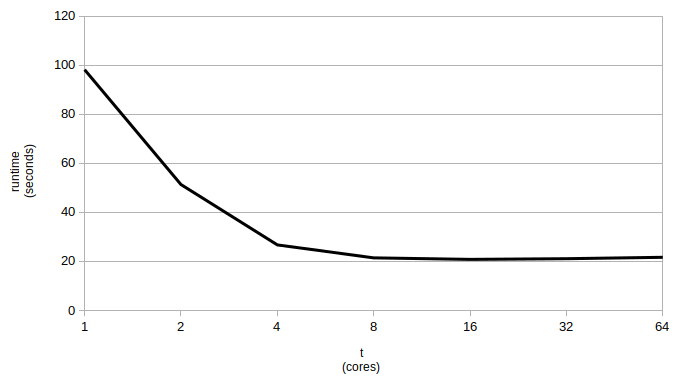
\includegraphics[width=0.8\textwidth]{chart01.png}
    \centering
    \caption{Line Chart of the Average runtimes of the computer program with 1 to 64 threads (multiprocessing)}
    \end{figure}


\indent As seen in Table 1, the running times of the code using different number of \emph{t} cores. As the number of cores increase, the runtimes decrease. This progression can be easily observed during the increasing of number of \emph{t} cores while dealing with low values, but as the number of cores increase, the decrease in runtime flattens as it continues.\\
\indent To compare the recently obtained data to the previously obtained data using multithreading in the previous exercise, the table from the previous laboratory report is shown below:

\begin{table}[H]
    \centering
    \noindent\makebox[\textwidth]{
    \begin{tabular}{|c|c|ccc|c|}
    \hline
    \multirow{2}{*}{\textbf{\begin{tabular}[c]{@{}c@{}}n\\ (size of matrix)\end{tabular}}} & \multirow{2}{*}{\textbf{\begin{tabular}[c]{@{}c@{}}t\\ (number of concurrent threads)\end{tabular}}} & \multicolumn{3}{c|}{\textbf{\begin{tabular}[c]{@{}c@{}}Time Elapsed\\ (seconds)\end{tabular}}} & \multirow{2}{*}{\textbf{\begin{tabular}[c]{@{}c@{}}Average Runtime\\ (secs)\end{tabular}}} \\ \cline{3-5}
                                                                                           &                                                                                                      & \multicolumn{1}{c|}{\textbf{Run 1}}   & \multicolumn{1}{c|}{\textbf{Run 2}}  & \textbf{Run 3}  &                                                                                            \\ \hline
    8000                                                                                   & 1                                                                                                    & \multicolumn{1}{c|}{100.912083}       & \multicolumn{1}{c|}{99.045359}       & 98.716483       & 99.557975                                                                                  \\ \hline
    8000                                                                                   & 2                                                                                                    & \multicolumn{1}{c|}{106.021552}       & \multicolumn{1}{c|}{107.055136}      & 105.227246      & 106.101311333333                                                                           \\ \hline
    8000                                                                                   & 4                                                                                                    & \multicolumn{1}{c|}{108.299674}       & \multicolumn{1}{c|}{107.104734}      & 107.16318       & 107.522529333333                                                                           \\ \hline
    8000                                                                                   & 8                                                                                                    & \multicolumn{1}{c|}{114.795173}       & \multicolumn{1}{c|}{113.608294}      & 122.527366      & 116.976944333333                                                                           \\ \hline
    8000                                                                                   & 16                                                                                                   & \multicolumn{1}{c|}{119.669082}       & \multicolumn{1}{c|}{118.507086}      & 119.356774      & 119.177647333333                                                                           \\ \hline
    8000                                                                                   & 32                                                                                                   & \multicolumn{1}{c|}{124.609196}       & \multicolumn{1}{c|}{124.346253}      & 122.94652       & 123.967323                                                                                 \\ \hline
    8000                                                                                   & 64                                                                                                   & \multicolumn{1}{c|}{125.016126}       & \multicolumn{1}{c|}{130.814412}      & 125.503346      & 127.111294666667                                                                           \\ \hline
    \end{tabular}}
    \caption{\label{table}Average runtimes of the computer program from 1 to 64 concurrent threads (multithreading)}
    \end{table}

\indent In comparing Tables 1 and 2, it is observed that the trend in both tables are different. The table obtained in Table 2 shows an inverse relationship with the \emph{n} size of matrix and \emph{t} number of threads, while Table 1 displays a direct relationship with the \emph{n} size of matrix and \emph{t} number of threads.\\
\indent The reason for the difference in trends in tables of multiprocessing (Table 1) and multithreading (Table 2) is the Global Interpreter Lock (GIL) present when using the \emph{multithreading} module \cite{intro, gil}. GIL is being applied when dealing with muliple threads in Python, but not when using multiple processes. Hence, the decrease in runtime in multiprocessing, unlike in multithreading \cite{GIL-thread}.

\begin{figure}[H]
    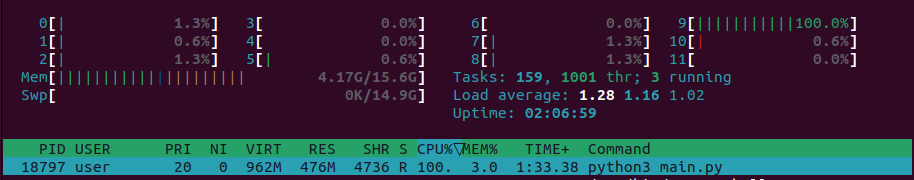
\includegraphics[width=0.8\textwidth]{table01.png}
    \centering
    \caption{Screen capture of \emph{htop} during the execution of the computer program using a single thread}
    \end{figure}

\begin{figure}[H]
    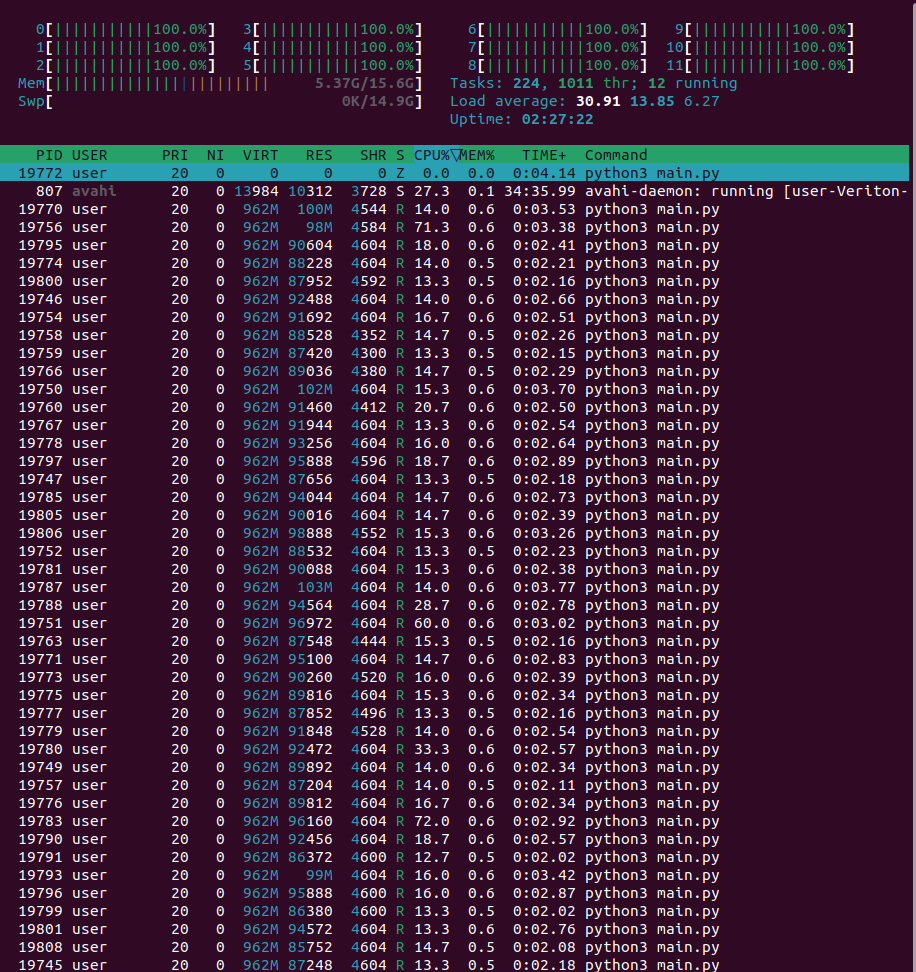
\includegraphics[width=0.8\textwidth]{table07.png}
    \centering
    \caption{Screen capture of \emph{htop} during the execution of the computer program using 64 threads}
    \end{figure}

\indent Figures 2 and 3 shows the screen captures of \emph{htop} while running the program. The CPU\% column shows what percentage of the capacity of the memory is being utilized by the process \cite{htop}. In Figure 2, it is seen that a single core is being maximized. And in Figure 3, all cores are being maximized during runtime.

\section*{Conclusion}
\hspace{\parindent} The complexity of estimating the point elevation of a \emph{n $\times$ n} square matrix with randomized values at grid points divisible by 10 when using n concurrent threads is O(n) because each column is iterated through only once, since each column will be assigned to a single thread, which will be then be assigned to a core. This complexity is still the same with the multithreading program, but since GIL is not being utilized in the \emph{multiprocessing} module of Python, the speedup is observed.\\
\indent Compared to Exercise 01 and 02, the runtimes obtained in this exercise is much faster. This also made it possible for higher \emph{n $\times$ n} square matrices to be possible to be interpolated since the GIL is now hindering the processes in running concurrently. 


\printbibliography{}


\pagebreak
\section*{\centering Appendix}
\begin{center}
Interpolation Source Code \\ (main.py)
\end{center}
\setstretch{1}
\begin{lstlisting}[language=Python]
    import numpy as np
    import random
    import datetime
    import os
    import threading
    from multiprocessing import Process


    print("This machine has", os.cpu_count(),"number of CPUs")

    # prettier printing options
    np.set_printoptions(linewidth=1000, formatter={'float': '{: 0.0f}'.format})



    # interpolate function
    def terrain_inter_multithreading(mat,x1,x2):
        for i in range(0,n):
            for j in range(x1,x2):
                if mat[i][j] != 0:
                    continue
                if (i % dist == 0):
                    get_row_val(i,j)
        for i in range(0,n):
            for j in range(x1,x2):
                if (mat[i][j] == 0):
                    get_col_val(i,j)

    # modified interpolation function
    # to run concurrently with other threads
    # from other x1 to x2's
    def terrain_inter_multiprocessing(mat,x1,x2):
        for i in range(0,n):
            for j in range(x1,x2+2):
                if mat[i][j] != 0:
                    continue
                if (i % dist == 0):
                    get_row_val(i,j)
        for i in range(0,n):
            for j in range(x1,x2+2):
                if (mat[i][j] == 0):
                    get_col_val(i,j)

    def get_submatrices(n,t):
        # array of submatrices
        sub_arr = []
        temp = []
        for i in range(0,n):
            temp.append(i)
            if (len(temp) == (n-1) / t):
                sub_arr.append(temp)
                temp = []

        return sub_arr

    # get size of matrix
    def getSize():
        n = 1
        while (n % 10 != 0):
            n = int(input("enter size of matrix: "))
            if n % 10 != 0:
                print('invalid size of matrix')
        return n+1

    # get number of threads
    def getThreads(n):
        n -= 1
        t = 0
        # n size should be less than t threads
        # t threads should not be 0
        # n size should be divisible by t threads
        while (n < t) or (t == 0) or (n % t != 0):
            t = int(input('enter number of threads: '))
            if (n < t) or (n % t != 0):
                print('invalid number of threads')
        return t

    def getCores(n):
        n -= 1
        t = 0
        # n size should be less than t threads
        # t threads should not be 0
        # n size should be divisible by t threads
        while (n < t) or (t == 0) or (n % t != 0):
            t = int(input('enter number of threads: '))
            if (n < t) or (n % t != 0):
                print('invalid number of threads')
        return t

    # dp array format:
    # dp = [[x1,y1][x2,y2]]

    # interpolate rows with random values
    def get_row_val(i,j):
        dp = get_datapoints_row(i,j)
        x = j               # j -> row
        x1 = dp[0][0]
        x2 = dp[1][0]
        y1 = dp[0][1]
        y2 = dp[1][1]
        res = fcc(x1,y1,x2,y2,x)
        mat[i][j] = res

    # interpolate columns
    def get_col_val(i,j):
        dp = get_datapoints_col(i,j)
        # dp = [[x1,y1][x2,y2]]
        x = i               # i -> col
        x1 = dp[0][0]
        x2 = dp[1][0]
        y1 = dp[0][1]
        y2 = dp[1][1]
        res = fcc(x1,y1,x2,y2,x)
        mat[i][j] = res


    # get closest datapoints to the current gridpoint
    def get_datapoints_row(i,j):
        dp = []
        dp.append(get_nearest_row(i,j,-1))
        dp.append(get_nearest_row(i,j,+1))
        return dp
    def get_datapoints_col(i,j):
        dp = []
        dp.append(get_nearest_col(i,j,-1))
        dp.append(get_nearest_col(i,j,+1))
        return dp

    # x, y -> point; dir -> direction 
    # change direction to check to the nearest 10
    ## improved from recursion from previous exercise to direct computation
    def get_nearest_row(i,j,dir):
        # go up
        if dir < 0:
            dir = j - (j % 10)
        # go down
        else:
            dir = j + (10 - (j % 10))
        return [dir,mat[i][dir]]

    def get_nearest_col(i,j,dir):
        # go left
        if dir < 0:
            dir = i - (i % 10)
        # go right
        else:
            dir = i + (10 - (i % 10))
        return [dir,mat[dir][j]]

    # follow given FCC formula
    def fcc(x1,y1,x2,y2,x):
        return (y1 + (((x-x1)/(x2-x1)) * (y2-y1)))

    # main function
    if __name__ == "__main__":
        # initialize data
        n = getSize()
        t = getCores(n)

        # distance between randomized values
        dist = 10

        # create a zero nxn matrix
        mat = np.zeros((n,n), dtype = float)

        # randomize elevation values for gridpoints divisible by 10
        for i in range(n):
            for j in range(n):
                if i % dist == 0 and j % dist == 0:
                    mat[i][j] = random.uniform(0.0, 1000.0)

        # print initial matrix
        print(mat)

        threads = list()

        for set in get_submatrices(n,t):
            x1, x2 = set[0], set[-1]
            thread = threading.Thread(target=terrain_inter_multithreading, args=(mat,x1,x2))
            threads.append(thread)

        # record time before threaded interpolation
        time_before_multithreading = datetime.datetime.now()


        for thread in threads:
            thread.start()

        for thread in threads:
            thread.join()

        # record time after threaded interpolation
        time_after_multithreading = datetime.datetime.now()
        # print resulting matrix
        print(mat)

        print("\n\n\n")


        # create a zero nxn matrix
        mat = np.zeros((n,n), dtype = float)

        # randomize elevation values for gridpoints divisible by 10
        for i in range(n):
            for j in range(n):
                if i % dist == 0 and j % dist == 0:
                    mat[i][j] = random.uniform(0.0, 1000.0)

        # print initial matrix
        print(mat)

        processes = list()

        for set in get_submatrices(n,t):
            x1, x2 = set[0], set[-1]
            process = Process(target=terrain_inter_multiprocessing, args=(mat,x1,x2))
            processes.append(process)

        # record time before threaded interpolation
        time_before_multiprocessing = datetime.datetime.now()


        for process in processes:
            process.start()

        for process in processes:
            process.join()

        # record time after threaded interpolation
        time_after_multiprocessing = datetime.datetime.now()


        # print resulting matrix
        print(mat)

        # print interpolation time
        print("multithreading: ",time_after_serial-time_before_serial)
        print("multiprocessing: ",time_after_multiprocessing-time_before_multiprocessing)
\end{lstlisting}

\end{document}
